% !TeX root = ../main.tex
% Add the above to each chapter to make compiling the PDF easier in some editors.

\chapter{Evaluation}\label{chapter:evaluation}
Our original goal was to bring a first prototype fuzzer to the Algorand ecosystem of tools and for this reason we designed and implemented AlgoFuzz.
In this chapter, we will evaluate AlgoFuzz to see if it fulfills its purpose as a fuzzer.
The most straightforward way to find out if a fuzzer works is to see if it is able to find bugs, known and unknown.
Looking at other smart contract fuzzers, such as ContractFuzzer or Harvey, we can see that the most common approach is to run the fuzzer on real-world contracts.
After which they would see if their fuzzer reported any bugs during the process.
In our case, since we are dealing with a property-based fuzzer and we do not have a list of predefined bug oracles, we would need to know the contracts in detail to be able to write properties that would find bugs.
Echidna, the property-based fuzzer for Ethereum, was also faced with this problem.
Instead of finding bugs, they decided to see if their fuzzer was able to reach certain assertion failures which were randomly added to the contracts.

With these considerations in mind we came up with two different questions that we wanted to answer for our evaluation:
\begin{enumerate}
    \item[\textbf{RQ.1}] How does the code coverage evolve over time, especially during prolonged fuzzing sessions?

    \item[\textbf{RQ.2}] How effectively can AlgoFuzz discover the state space of the smart contract?
\end{enumerate}

\section{Setup}

\subsection*{Chosen Contracts}
For our evaluation, it was difficult to find real-world Algorand smart contracts which adhered to the limitations of our fuzzer namely using the official \ac{ABI}, not using any box state and not interacting with \acp{ASA}.
For this reason we decided to write our own contracts in PyTeal based on already existing Solidity smart contracts which where used in previous works.
The first set of contracts we chose were the twelve contracts used in the Echidna evaluation \cite{grieco_echidna_2020}, namely a subset of the VeriSmart-benchmarks \cite{noauthor_kuplverismart-benchmarks_nodate}.
For our second set of contracts we chose two contract of a larger size than the ones selected before.
The first one being the Tether stablecoin contract, presented in our case study in \ref{section:case-study}.
The second one a generic token exchange contract, where the user can buy and sell tokens for Algos given an exchange rate.

\subsection*{Evaluation Protocol}
The metrics we gathered for our experiments were the ones mentioned in section \ref{section:metrics}.
We ran each configuration of the fuzzer as we did in the case study, so six configurations in total (two different fuzzing strategies and three different fuzzing drivers).
For the 12 small contracts we did 10 runs per configuration with a fuzzing time of 10 minutes each.
In total the fuzzer ran for these contracts for 120 hours.
The two larger contracts also ran for 10 times per configuration but with a fuzzing time of 30 minutes each.
For the larger contracts the fuzzer ran in total for 60 hours.
All in all the experiment ran for 180 hours. After each call to the target contract we recorded the metrics in a \acs{CSV} file. The results that we show are the average of the 10 runs for each configuration.

The experiments were run on a virtual machine hosted on the LRZ Compute Cloud \cite{noauthor_lrz_nodate}.
The compute node uses Intel(R) Xeon(R) Gold 6148 CPUs at 2.40GHz.
The virtual machine had 2 CPU cores, 9 GB of RAM and 30 GB of disk space.
The operating system was Ubuntu 20.04 LTS.
AlgoFuzz used the Python 3.10.12 interpreter, the Algorand node was version 3.15.1, and the Docker version was 24.0.6.

\section{Results}
In this section we will present the quantitative results of our evaluation.
We also elaborate on how the data was selected and transformed to be able to present it in a meaningful way.

From the data we collected we excluded some runs which were uncharacteristically slow, assuming that they were statistical outliers caused by the virtual machine.
The runs we excluded were the ones where the number of calls was much lower than the average for the same configuration.
These happened to be runs on the AlgoTether contract with the Total Fuzzer and the Coverage driver.

We wanted to gather the aggregate data of each configuration per call, so for our graphs we took as maximum number of calls the minimum number of calls of the runs in the same configuration.
For example if we had run 1 with 10 calls, run 2 with 20 calls and run 3 with 15 calls, we would only take the first 10 calls of each run.
As we mentioned that most runs had almost the same number of calls, this did not affect the results in a significant way.
After this we calculated the average, median, minimum and maximum of each metric for each call.
We used this to graph the different metrics over the number of calls.
In our graphs we will only be presenting the values of the larger contracts, since the smaller contracts reach a saturation point very quickly and they do not change significantly after that.

Aside from that we also calculated the values for the last call of each run to see what the final state of the fuzzer was.

\subsection*{Code Coverage}
To answer \textbf{RQ.1} we will look at percentage of code coverage over the number of calls to the target contract.
Other metrics such as the number lines covered or the number of unique paths covered were also considered but were discarded since they did not provide any additional information.
The reason for this is because these metrics are correlated with each other and the graphs looked very similar.
The advantage of using the percentage of code coverage is that it is a normalized metric and it is easier to compare the results of different contracts.


\begin{figure}[htbp]
    \centering
    \subfloat[AlgoTether][AlgoTether]{
        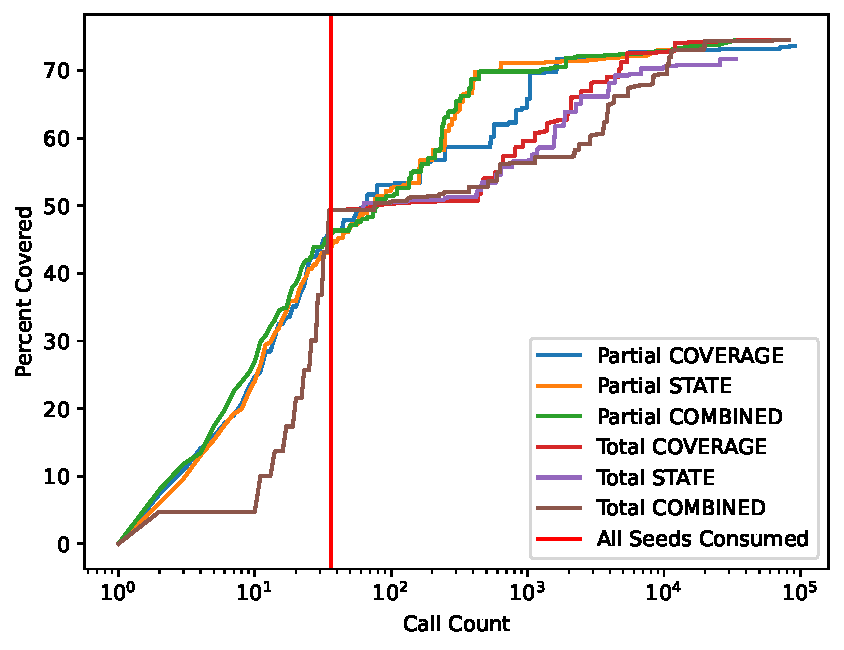
\includegraphics[width=0.48\textwidth]{charts/AlgoTether_ percent_covered_seed.pdf}
        \label{fig:AlgoTether_cov}
    }
    \hfill
    \subfloat[ExchangeToken][ExchangeToken]{
        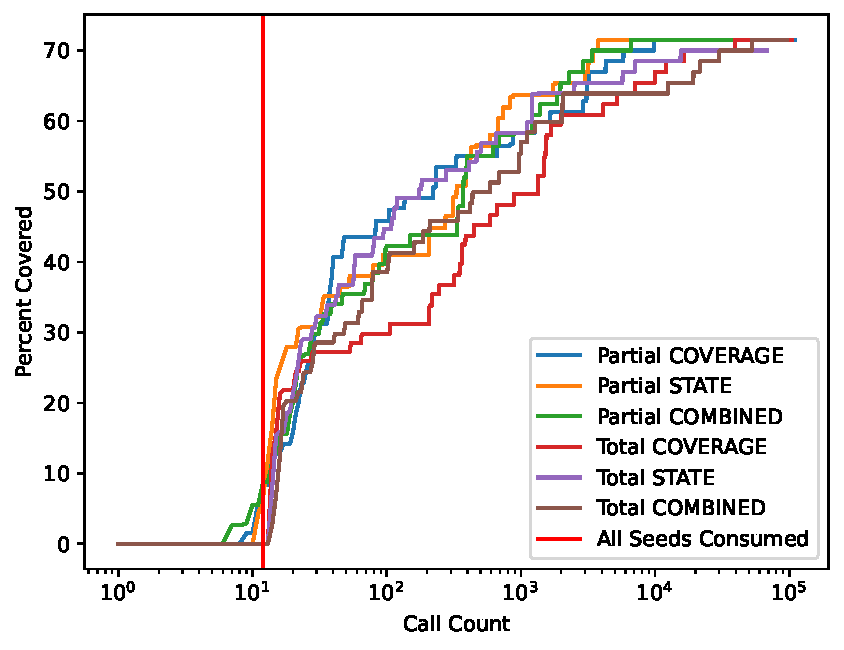
\includegraphics[width=0.48\textwidth]{charts/ExchangeToken_ percent_covered_seed.pdf}
        \label{fig:ExchangeToken_cov}
    }
    \caption{Average coverage of AlgoTether and ExchangeToken for all configurations.}
    \label{fig:percent_coverage}
\end{figure}

In Figure \ref{fig:percent_coverage} we can see the percentage of code coverage over the number of calls for the two larger contracts.
The x axis which represents the number of calls is shown in logarithmic scale.
This is because coverage increases very quickly in the beginning and then it slows down.
All the different configurations are shown in the same graph to be able to compare them.
We can observe that the Total Fuzzer, in both cases regardless of the driver, lags behind the Partial Fuzzer.

Another interesting observation is that the fuzzer behaves very differently for the two contracts in the early stages.
For the AlgoTether contract, the fuzzer immediately covers new code on almost every call for while consuming the seeds.
On the other hand, for the ExchangeToken contract, most of the seed values do not cover new code.
We also graphed the ranges and the medians of the coverage for each contract, which can be seen in Figure \ref{fig:AlgoTether range} and Figure \ref{fig:ExchangeToken range} respectively.
In these graphs can be seen that the coverage has no variance in the beginning for the Total fuzzer, while the Partial fuzzer has a lot of variance depending on the driver.

In Table \ref{table:covs-noseed-acc} we can see the final code coverage for each contract after we remove the coverage gained by the seed inputs.
Aside from contracts 1, 4, and 12, in all other contracts the fuzzers have gained coverage beyond what was covered by the seeds.
Table \ref{table:covs} shows us that almost all fuzzers achieved the maximum coverage.
The only exception being the Total State fuzzer on the AlgoTether, ExchangeToken and '019' contracts, and Partial Coverage fuzzer on the AlgoTether contract.


\begin{table}[htbp]
    \centering
    \csvautotabular{data/covs-noseed-acc.csv}
    \caption{Final code coverage for each contract subtracting seed coverage.}\label{table:covs-noseed-acc}
\end{table}
